% Primarily this section should be about scientific methods and theories you need to evaluate/compare/invent to solve your problems from 1.3.
% In some cases it may be ok to describe different technologies, but the purpose is to describe something and then draw a conclusion from that.
% Example, if you decide to discuss different databases, it may be for the purpose of selecting the best type for your implementation later on (based on for example data representation, scalability, speed, etc.).
% Optimally the problems in 1.3 are not solved by anyone else yet, in which case this section needs to describe how to solve them (new algorithms, mathematical approaches, etc.).
 
% This chapter can have a lot of sections (3.1, 3.2, 3.3, etc).

\section{Registers and Memory}
\label{sec:regmem}
The two main places a computer stores values are in registers or the memory.
Registers are very limited in space and are very volatile.
Volatile, in this case, means that new values get written to the register often.
Therefore, registers are suitable for storing values used many times in a concise amount of time.
Memory is much slower but has a lot more space.
Therefore, it is better for storing long-lived values.


The compiler decides when and where values are stored, and it decides this during the compilation of the program.
Therefore, the developer has little control over where the values are stored.


Values located in memory are either stored on the call stack or the heap.
The call stack holds all the values of arguments and variables for all the called functions that have not finished execution.
In contrast, the heap contains all the dynamically allocated values.


\subsection{Registers}
Computer registers are small memory spaces that are of fixed size.
These registers can store any data if it fits within the size limit.
Some registers are reserved for a particular use.
The \acrfull{pc} register is among the most important and contains the succeeding machine code instructions to be executed.
The registers reserved for a particular use differ depending on the processor architecture.


\subsection{Call Stack}
\label{sec:callstack}
The call stack consists of each function call that has not terminated.
A stack is a data structure consisting of several elements stacked on top of each other, and the only two operations available for a stack are push and pop.
The push operations will add an element on top of the stack, and the pop operation removes the top element of the stack.
Another critical characteristic is that only the top element can be accessed; therefore, all the above elements need to be popped to reach the lower elements.



Stack/call frames are the elements that make up the call stack.
Each stack frame contains the values of the arguments and variables for a function call, and stack frames usually contain a return address.
When a function is finished, the return address is written to the \acrshort{pc} register, making the program jump to the return address.
The return address usually points back to the previous function.
Also, when a function has finished executing, its stack frame will be popped/removed from the stack.
See figure \ref{fig:callstack} for an example of a call stack and stack frames.
The values starting with \emph{0x} to the right in the figure are hexadecimal addresses.


\begin{figure}[!htb]
	\centering
	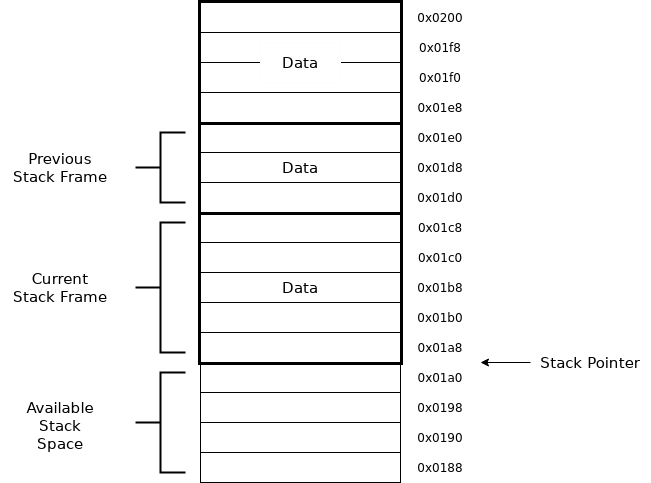
\includegraphics[width=1.0\textwidth]{call-stack.png}
	\caption{A visual example of how a stack and stack frames can look.}
	\label{fig:callstack}
\end{figure}



\section{Prologue and Epilogue Code}
Some registers need to be preserved during the execution of a subroutine.
The prologue code pushes those registers onto the call stack at the start of the subroutine.
At the end of the subroutine, the epilogue code pops the stored registers from the stack.
It is the compiler that generates the prologue and epilogue code.


Note that the prologue and epilogue code is only sometimes continuous blocks of code at the beginning and end of a subroutine. 
Read  \cite{dwarf} pages 126-127 to learn more about the prologue an epilogue.



\section{Debugging}
Debugging refers to the process of finding and resolving errors, flaws, or faults in computer programs.
A bug is an error, flaw, or fault in computer science.
Bugs are the cause of software behaving unexpectedly.
Most bugs arise from poorly written code, lack of communication between the developers, and lack of programming knowledge.


There are multiple methods to debug computer programs.
One of the most common methods is testing, which is done by sending some input to the code and comparing the result to the expected result.
The amount of code tested in a test can vary from one function to the whole program.
Another debugging method is a control flow analysis, which analyzes the order in which the instructions, statements, or function calls are.
There are many more methods to debug computer programs, but they all try to achieve the same thing.
That is, to give the programmer a deeper understanding of what is happening.


There is no better tool for understanding a program than a debugger.
That is because a debugger can display the state of a program, and it has control of its execution.
A debugger enables the inspection of every part of a program, which is especially true for modern debuggers with much more advanced features.


\subsection{Debugger}
A \emph{debugger} is a computer program used to test and debug other computer programs.
The two main functionalities of a debugger are, firstly, the ability to control the execution of the target program.
Secondly, it is the ability to inspect the state of the target program.


Some of the most common ways a debugger can control a target program are by continuing, halting, stepping, and resetting the execution.
Continuing the execution means that the target program continues the execution from the current stopped location.
Halting the target program can often be done in two ways, the first is to stop the execution where it currently is, and the other way is to set a breakpoint.
A breakpoint is a point in the code that, if reached, will stop the target program immediately.
Breakpoints are very useful for inspecting specific points in the code, while the other way of halting is used more when the location is unknown.
Stepping in the process of continuing the target program execution for only a moment, often just until the following source code line is reached, there are many stepping variants.
Lastly, resetting means that the target program will start execution from the beginning.


Most debuggers display the state of the target program relative to the source code.
Therefore, if the target program has halted, the closest source code location will be shown as the halt location.
They also often let the user set the breakpoint in the source code and translate that to the closest machine code instruction.
Other features most debuggers have is the ability to show a stack trace, variables (type and value), and evaluate an expression.
There are a lot more functionalities that a debugger can have, but these are some of the most common ones.


\section{DWARF}
\label{sec:dwarf}
This section will explain how the debug information format \acrfull{DWARF} version $4$ is structured and what functionality the different sections have.
However, it will not explain every detail about the \gls{DWARF} format because the \gls{DWARF} specification already does that.
Instead, this section will focus on the type of information stored in the \gls{DWARF} format and how to use it.
For more details, see the \gls{DWARF} specification \cite{dwarf}.


\subsection{Dwarf Sections}
The \gls{DWARF} format consists of sections containing different information.
Pointers consisting of different offsets connect some sections.
Many \gls{DWARF} attributes contain these offsets. See section \ref{sec:dwarfattributes} for information about attributes.
Figure \ref{fig:dwarfsections} shows the \gls{DWARF} sections and which ones point to each other.
All \gls{DWARF} sections are stored in an \gls{elf} file, a binary file format divided into different sections.
The \gls{elf} format contains a table describing what each of its sections contains and where they begin and end.


\begin{figure}[h]
	\centering
	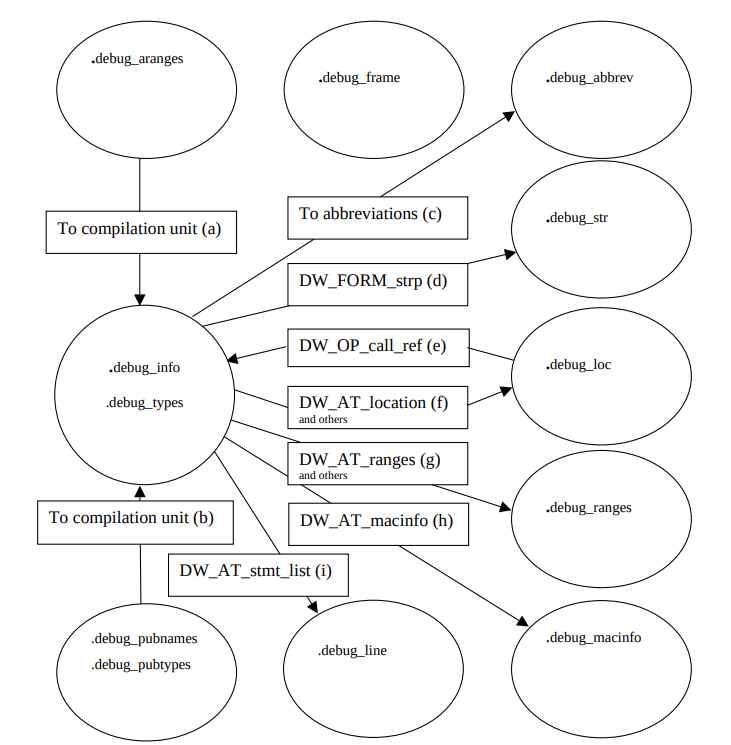
\includegraphics[width=0.9\textwidth]{dwarf-sections}
	\caption{Diagram of the different \gls{DWARF} sections and their relations to each other.}
	\label{fig:dwarfsections}
\end{figure}


\subsubsection{\emph{.debug\_abbrev}}
The \gls{DWARF} section \emph{.debug\_abbrev} contains all the abbreviation tables used to translate abbreviation codes into their official \gls{DWARF} names.
Abbreviation codes are used in \acrfull{die} tags, \gls{die} attribute names, and more.
An abbreviation code is translated by looping through the entries in one of the abbreviation tables until it finds the matching one.
For further details, we refer the reader to section $7.5.3$ in \cite{dwarf}.


\subsubsection{\emph{.debug\_aranges}}
All the information needed to look up compilation units using machine code addresses is in the \gls{DWARF} section \emph{.debug\_aranges}.
Compilation units contain debugging information for a range of machine code addresses.
Each compilation unit has a start address followed by a length.
Therefore, to find the correct compilation unit, the user only needs to check if the current address is between the start address and the start address plus the length.
For further details, we refer the reader to section $6.1.2$ in \cite{dwarf}.


\subsubsection{\emph{.debug\_frame}}
In the \gls{DWARF} section \emph{.debug\_frame}, the information needed to unwind the call stack virtually is kept.
It consists of two structures named \acrfull{cie} and \acrfull{fde} and is entirely self-contained.
Virtually unwinding the call stack is complex.
Therefore, for further details, we refer the reader to section \ref{sec:stacktrace} in this document and section $6.4.1$ in \cite{dwarf}.


\subsubsection{\emph{.debug\_info}}
Most of the information about the source code is in \glspl{die} which are a low-level representation of the source code.
\glspl{die} have a tag that describes what it represents.
An example tag is \emph{DW\_TAG\_variable}, meaning that the \gls{die} represents a variable from the source code.
All \glspl{die} are stored in trees.
Each one of the trees is a \gls{DWARF} compilation unit or a partial one.
The trees are structured the same as the source code, which makes it easy to relate the source code to the machine code.
The section \emph{.debug\_info} consists of several \gls{DWARF} units and other debug information.
Therefore, this is one of the most valuable sections in \gls{DWARF} because it contains the relation between the state of the debug target and the source code and vice versa.


\subsubsection{\emph{.debug\_line}}
The \gls{DWARF} section \emph{.debug\_line} holds the needed information to find the machine addresses generated from a specific line and column in the source file.
It contains the source directory, file name, line number, and column number.
Pointers to this information are in some \glspl{die}.
Therefore, enabling the debugger to get the source location of a \gls{die}.
Section $6.2$ in \cite{dwarf} explains more about the information in the \emph{.debug\_line} section.


\subsubsection{\emph{.debug\_loc}}
The location of the variables is in location lists, which are in the \emph{.debug\_loc} section.
Each location list entry holds several operations that, when performed, will yield the location of a value.
Some \glspl{die} in the \emph{.debug\_info} section have attributes that point to entries in the location lists.
The most common of these attributes is named \emph{DW\_AT\_location}, which is often present in \glspl{die} representing variables.
See figure \ref{fig:dwarfsections} for a graph showing the relationship between these two sections.


\subsubsection{\emph{.debug\_macinfo}}
The \emph{.debug\_macinfo} section contains all the macro information stored in entries representing the macro after the compiler has expanded it.
Some \glspl{die} in the \gls{DWARF} section \emph{.debug\_info} point to these entries, and those pointers are in the \glspl{die} attribute \emph{DW\_AT\_macinfo}.
For further information, we refer the reader to section $6.3$ in \cite{dwarf}.


\subsubsection{\emph{.debug\_pubnames} and \emph{.debug\_pubtypes}}
There are two sections for looking up compilation units by the name of functions, variables, types, and more.
The first is \emph{.debug\_pubnames}, which is for finding functions, variables, and objects, and the other is for finding types.
This section is named \emph{.debug\_pubtypes}.
For further details, we refer the reader to section $6.1.1$ in \cite{dwarf}.


\subsubsection{\emph{.debug\_ranges}}
\glspl{die} with a set of non-contiguous addresses will have an offset to the section \emph{.debug\_ranges} instead of an address range.
The offset points to the start of a range list containing range entries, which are for knowing which of the machine code addresses the \gls{die} is active.
The \gls{DWARF} section \emph{.debug\_ranges} is for storing these lists of ranges.
For further details, we refer the reader to section $2.17$ in \cite{dwarf}.


\subsubsection{\emph{.debug\_str}}
The DWARF section \emph{.debug\_str} is for storing all the debug information strings.
An example of these strings is the names of the functions and variables.
\glspl{die} representing variables and functions will have an offset that points to these strings in the attribute \emph{DW\_AT\_name}. 


\subsubsection{\emph{.debug\_type}}
The \gls{DWARF} section \emph{.debug\_type} is similar to section \emph{.debug\_info} in that it is also made up of compilation units, with each a tree of \glspl{die}.
The difference is that the \glspl{die} are a low-level representation of the types in the source code.



% Explain DWARF Unit
\subsection{Dwarf Compilation Unit}
When compiling a source program, the compiler will mainly generate one compilation unit for each project/library.
There are some cases when it generates multiple partial compilation units instead.
The compilation units are in the \gls{DWARF} section \emph{.debug\_info}.
These compilation units are structured the same as the source code, which makes it easy to relate between the debug target state and the source code.


The first \gls{die} in the tree of the compilation unit will have the tag \emph{DW\_TAG\_compile\_unit}.
This \gls{die} has many valuable debug information about the source file, one being the compiler used and its version.
It also says which programming language the source file is in as well as the directory and path of the source file.



\subsection{Dwarf Debugging Information Entry}
One of the most important data structures in the \gls{DWARF} format is the \gls{die}.
A \gls{die} is a low-level representation of a small part of the source code.
The most common source code objects that the \glspl{die} represent are functions, variables, and types.
The \glspl{die} are in a tree structure called a \gls{die} tree.
Each \gls{die} tree will often represent a whole compile unit or all types used in the source code.
The ones representing compile units are found in the \gls{DWARF} section \emph{.debug\_info}, while the ones representing type are in the \gls{DWARF} section \emph{.debug\_type}.
The \glspl{die} representing types are named type \glspl{die}.


\subsubsection{Dwarf Attribute}\label{sec:dwarfattributes}
All the information stored in \glspl{die} is in unique attributes.
These attributes consist of a name and a value.
The attribute's name is unique and describes what type of information the attribute's value has.
All the attribute names start with \emph{DW\_AT\_}, and then some name that describes the attribute.
An example is the name attribute \emph{DW\_AT\_name}. 
In the \gls{DWARF} file, the name of the attributes is abbreviated to its abbreviation code which can be decoded using the \emph{.debug\_abbrev} section.


\subsubsection{Example of a DIE}
Figure \ref{fig:dwarfdie} shows an example of a \gls{die}.
The figure is a screenshot of the output from the program \emph{objdump} run on an \gls{elf} file.
The first line in the figure begins with the number $8$, representing the depth in the \gls{die} tree where this \gls{die} is located.
The following number is the current offset into this compile unit.
All the other lines in the figure also start with their offset.
Then comes \emph{"Abbrev Number: $9$"} on the same line.
It is an abbreviation code that translates to \emph{DW\_TAG\_variable}.
This tag means that the \gls{die} represents a variable from the source code.


\begin{figure}[h]
	\centering
	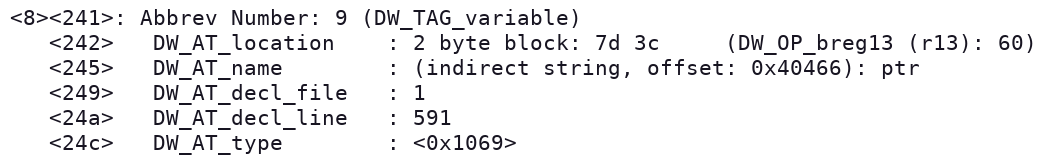
\includegraphics[width=1.0\textwidth]{dwarf-die.png}
	\caption{An example of a \gls{die} representing a variable named \emph{ptr}. This example is the output of the tool \emph{objdump} run on an \gls{elf} file.}
	\label{fig:dwarfdie}
\end{figure}


The attribute \emph{DW\_AT\_location} (seen in figure \ref{fig:dwarfdie}) has information about where the variable is stored on the debug target.
The attribute \emph{DW\_AT\_name} has an offset into the \gls{DWARF} section \emph{.debug\_str} that the \emph{objdump} tool has evaluated to ``str'', which is the variable's name.
Attributes \emph{DW\_AT\_decl\_file} and \emph{DW\_AT\_decl\_line} in the figure contain offsets into the section \emph{.debug\_line}.
Those offsets can be used to find the source file path and the line number from which the \gls{die} was generated.
Lastly, the attribute \emph{DW\_AT\_type} contains an offset into the section \emph{.debug\_types}, which points to a type \gls{die} that has the type information for this variable.


\subsection{Evaluate Variable}
\label{sec:evaluate-variable}
Evaluating a variable's value is complicated because there are many data types and combinations of data types.
Therefore, the following example is presented to simplify the explanation.


In the example, in figure \ref{fig:subprogramexample}, there is a function/subprogram \gls{die} with the name \emph{my\_function} (it is the \gls{die} with the tag \emph{DW\_TAG\_subprogram}).
The function has a parameter named \emph{val}, which is the \gls{die} with the tag \emph{DW\_TAG\_formal\_parameter}.
It is a child of the function \gls{die}, which means that it is a parameter to the function \emph{my\_function}.
This parameter \emph{val} will be used as an example of evaluating a variable.


\begin{figure}[h]
	\centering
	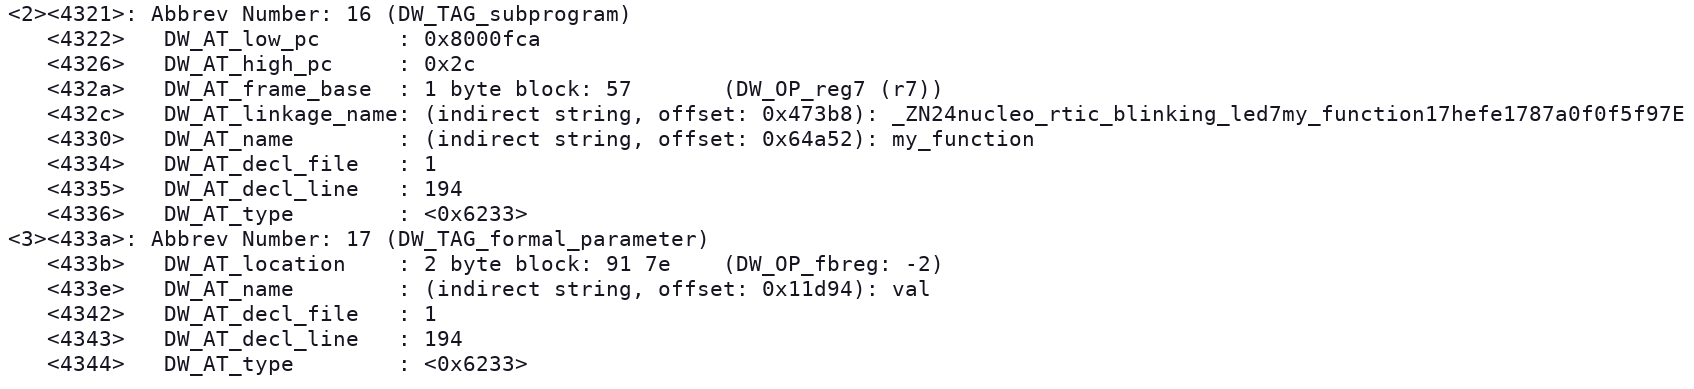
\includegraphics[width=1.0\textwidth]{subprogram-example.png}
	\caption{An example of a subprogram and parameter \gls{die}. This example is the output of the program \emph{objdump} run on an \gls{elf} file.}
	\label{fig:subprogramexample}
\end{figure}


Take note that the function \gls{die} named \emph{my\_function} has two attributes named \emph{DW\_AT\_low\_pc} and \emph{DW\_AT\_high\_pc}.
Those attributes describe the range of \gls{pc} values in which the function is executing.
Other attributes in the example will not be mentioned because they are not needed to determine the attribute's value.


\subsubsection{Finding Raw Value Location}
Examining the \gls{die} for the argument \emph{val}, there is an attribute named \emph{DW\_AT\_location}.
The value of that attribute is several operations, and performing these operations will give the location of the variable.


In this example, the operation in the \emph{DW\_AT\_location} attribute in figure \ref{fig:subprogramexample} is \emph{DW\_OP\_fbreg} -$2$.
That operation describes that the value is stored in memory at the \emph{frame base} minus $2$ (see \cite{dwarf} page 18).
The \emph{frame base} is the address to the first variable in the functions stack frame (see \cite{dwarf} page 56).


Currently, the value of the \emph{frame base} is unknown, but the location of the \emph{frame base} is described in the \emph{my\_function} \gls{die}.
The location of the \emph{frame base} is also described in several operations, and those operations are under the attribute \emph{DW\_AT\_frame\_base}.
Figure \ref{fig:subprogramexample} describes the \emph{frame base} location with the operation \emph{DW\_OP\_reg7}.
The operation \emph{DW\_OP\_reg7} describes that the value is located in register $7$ (see \cite{dwarf} page 27).
Therefore register $7$ needs to be read to get the value of the \emph{frame base}.


Now that the value of the \emph{frame base} is known, we can proceed to calculate the location of the parameter \emph{val}.
As mentioned previously, the location of parameter \emph{val} is the \emph{frame base} minus $2$.
Therefore, the value of \emph{val} can be read from memory at the address of the \emph{frame base} minus $2$.
However, the value must also be parsed into the type of \emph{val}.
See section \ref{sec:parsingvalue} for how to parse the value into the correct type.


\subsubsection{Parsing the Raw Value} \label{sec:parsingvalue}
The first problem with parsing the value of the parameter \emph{val} into the correct type is to know what type the parameter has, and this is where the attribute \emph{DW\_AT\_type} comes in.
The value of the \emph{DW\_AT\_type} attribute points to a type \gls{die} tree, which describes the type of the \gls{die}.


The offset to the type \gls{die} of the parameter val is $0x6233$, as shown in figure \ref{fig:subprogramexample}.
Finding that type \gls{die} is done by going to that offset in the \emph{.debug\_types} section.
  The type \gls{die} for \emph{val} can be seen in figure \ref{fig:basetypeexample}.
  Note that the offset of the \glspl{die} tag is the same as $0x6233$.
  That type \gls{die} has the tag \emph{DW\_TAG\_base\_type}, which means it is a standard type built into most languages (see \cite{dwarf} page 75).


\begin{figure}[h]
	\centering
	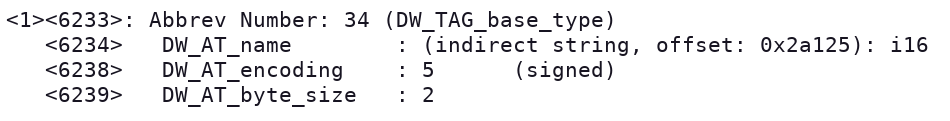
\includegraphics[width=1.0\textwidth]{basetype-example.png}
	\caption{An example of a base type \gls{die}. This example is the output of the program \emph{objdump} run on a \gls{elf} file.}
	\label{fig:basetypeexample}
\end{figure}


In this example, the type \gls{die} has three attributes that are used to describe the type.
The first attribute is \emph{DW\_AT\_name}, which describes the type's name.
In this case, the name of the type is \emph{i16}, which can be seen in figure \ref{fig:basetypeexample}.
The following attribute is \emph{DW\_AT\_encoding}, which describes the type's encoding.
Encoding with the value $5$ means that the type is a signed integer \cite{dwarf}.
The different values for encoding are specified in the \gls{DWARF} specification \cite{dwarf}.
The last attribute is \emph{DW\_AT\_byte\_size}, which describes the type size in bytes.
In this case, a byte size of $2$ means that the type is a $16$-bit signed integer.
The last step is to parse the bytes of the value into a signed $16$-bit integer.


\subsection{Virtually Unwind the Call Stack}
\label{sec:stacktrace}
The call stack is virtually unwinding by recursively unwinding a stack of \emph{subroutine activations}.
It is named virtual unwinding because the state of the debug target is not changed at any point during the unwinding.
Every subroutine in the call stack has an activation and a stack frame.
Because the activation often has the stack pointer value, the related stack frame is also known.
Therefore, successfully unwinding all the \emph{subroutine activations} will result in a complete understanding of the state of the call stack.


The debug information needed to unwind activations are stored in the \gls{DWARF} section \emph{.debug\_frame}.
That section is made up of two data structures.
One is named \gls{fde}.
An \gls{fde} contains a table used for unwinding registers and the \gls{cfa} of an activation.
The other data structure is named \gls{cie}.
It contains information that is shared among many \glspl{fde}.
The relevant \gls{cie} and \gls{fde} to an activation can be found using the \gls{pc} value.


Unwinding the stack of activation is done by first evaluating the values of the top activation.
See section \ref{sec:subact} to learn how that is done.
It starts with the top activation because too little information about the other activations is known.
The next step is to find the \gls{cie} and \gls{fde} that contain debug info on the subsequent activation.
When those are known, the values of the subsequent activation can be evaluated as described in section \ref{sec:subact}.
The unwinding is then repeated for the rest of the activations.


\subsubsection{Subroutine Activation} \label{sec:subact}
A \emph{subroutine activation} contains information on a subroutine call/activation.
Each \emph{subroutine activation} contains a code location within the subroutine, and it is the location where the subroutine stopped.
The reason for halting could be that a breakpoint was hit, it was interrupted by an event, or it could be the location where it made a call to the subsequent subroutine.


The address of the stopped code location is found using the stack pointer of the above activation in the activation stack.
That is because the return address of the above activation is the stopped code location of the current activation.
The return address is almost always stored on the stack.
Therefore, it can be read if the stack pointer is known.
It is true for all activations except for the top activation, where the current \gls{pc} value is the stopped code location.


An activation also describes the state of some registers where it stopped.
Those registers are preserved thanks to the prologue and epilogue code of the subroutine.
The rest of the registers are unknown because they have been written over, which makes them impossible to recover.


The activations are identified by their \gls{cfa} value.
The \gls{cfa} is the value of the stack pointer in the previous stack frame.
Note that the \gls{cfa} is not the same value as the stack pointer when entering the current \emph{call frame} (see \cite{dwarf} page 126).


The \gls{cfa} and the preserved register values can be restored using tables in the \gls{DWARF} section \emph{.debug\_frame}.
For further details, the reader is referred to section \ref{sec:evalcfa}.



\subsubsection{Unwinding CFA and Registers} \label{sec:evalcfa}
The tables in the \glspl{fde} contain virtual unwinding rules for a subroutine.
These virtual unwinding rules are used to restore the values of registers and the \gls{cfa}.


The first column in the tables contains code addresses.
Those addresses identify the code location to which all the row's virtual unwinding rules apply.
The next column is unique and contains the \gls{cfa}'s virtual unwinding rules. 
The remaining columns contain the virtual unwinding rules for registers $0$ to $n$, where n is the last registry.
See figure \ref{fig:stacktracetable} for a visual of how the tables are structured.


\begin{figure}[h]
	\centering
	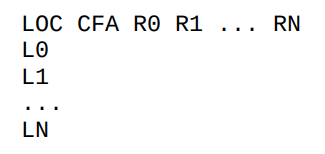
\includegraphics[width=0.5\textwidth]{stacktrace-table.png}
	\caption{This is how the table for reconstructing the \gls{cfa} and registers looks like. \emph{LOC} means that it is the column containing the code locations for $0$ to $N$. The column with \gls{cfa} has the virtual unwinding rules for \gls{cfa}. The rest of the column \emph{R0} to \emph{RN} holds all the virtual unwinding rules for the register $0$ to $N$.}
	\label{fig:stacktracetable}
\end{figure}


There are several virtual unwinding rules.
The ones for the registers are named register rules.
Some of them are easy to use, such as the register rule \emph{undefined}, and this rule means that it is impossible to unwind that register.
Other rules require calculations, such as the register rule \emph{offset(N)}, where the \emph{N} is a signed offset.
This rule means that the register value is stored at an address that can be calculated by adding the \gls{cfa} address and the offset \emph{N}.
All the rules can be read about in the \gls{DWARF} specification \cite{dwarf} on page 128.


Unwinding a register is done by first finding the correct row.
That is done by finding the row which contains the address that is closest but not greater than the current address.
The next step is to evaluate the new value using the register rule on the row, then go to the next row in the table and repeat but with the new value.
Repeat until there are no more rows.
That is how to use the table to unwind a register.
